\documentclass[hyperref={pdfpagelabels=true}]{beamer}

\usepackage{lmodern}
%%%%%%%%%%%%%%%%%%%%%%%%%%%%%%%%%%%%%%%%%%%%%%%%%%%%%%%%%%%%%%%%%%%%%%%%%%%%%%%%%%%%%%%%%%%%%%%%%
%This work is licensed under a Creative Commons Attribution-ShareAlike 4.0 International License.
%
%You are free to:
%
%    Share — copy and redistribute the material in any medium or format
%    Adapt — remix, transform, and build upon the material
%    for any purpose, even commercially.
%
%    The licensor cannot revoke these freedoms as long as you follow the license terms.
%
%Attribution — You must give appropriate credit, provide a link to the license, and indicate if changes were made. You may do so in any reasonable manner, but not in any way that suggests the licensor endorses you or your use.
%
%ShareAlike — If you remix, transform, or build upon the material, you must distribute your contributions under the same license as the original. 
%
%%%%%%%%%%%%%%%%%%%%%%%%%%%%%%%%%%%%%%%%%%%%%%%%%%%%%%%%%%%%%%%%%%%%%%%%%%%%%%%%%%%%%%%%%%%%%%%%%

\title{A GEO-stack for Big Data}
\subtitle{ Driving Spatial Analysis Beyond the Limits of
Traditional Storage}
\author{Joana Sim\~{o}es} 

\author[shortname]{Joana Sim\~{o}es \inst{1}}
\institute[shortinst]{\inst{1} BDigital, CASA, CICS.NOVA}

%\date{\today} 
\titlegraphic{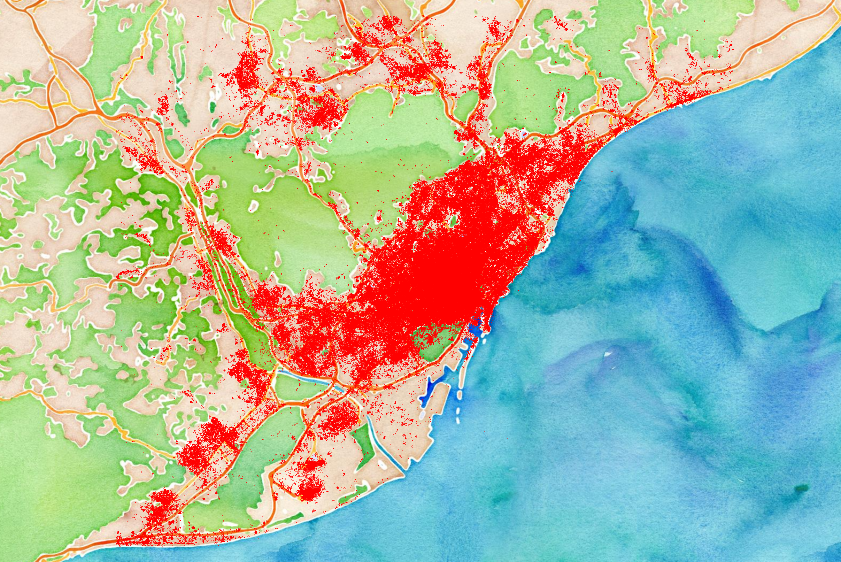
\includegraphics[width=.35\textwidth]{bigdata2.png}}
 
\usepackage{beamerthemeshadow}
%\usepackage{beamerthemesplit}
\usepackage{listings}

\newcommand{\soooo}{H$_2$SO$_4$}

%fdl stuff
\usepackage{hyperref}
\hypersetup{colorlinks, 
           citecolor=black,
           filecolor=black,
           linkcolor=black,
           urlcolor=black,
           bookmarksopen=true,
           pdftex}

\hfuzz = .6pt % avoid black boxes

\lstset{language=SQL}

\begin{document}
\setbeamertemplate{footline}[page number]
\setbeamertemplate{navigation symbols}{}
\begin{frame}
\titlepage

%\begin{titlepage}
%\centering{ 
%  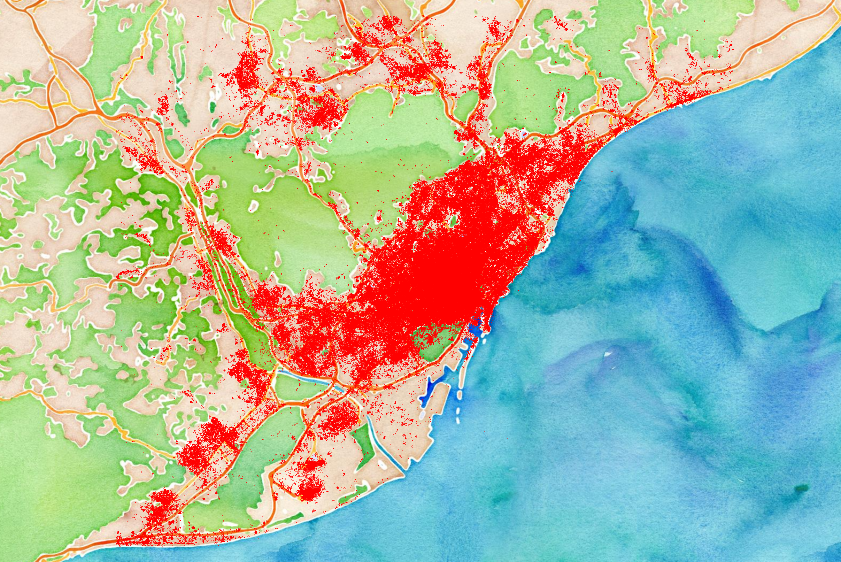
\includegraphics[scale=0.2]{bigdata2.png}
%  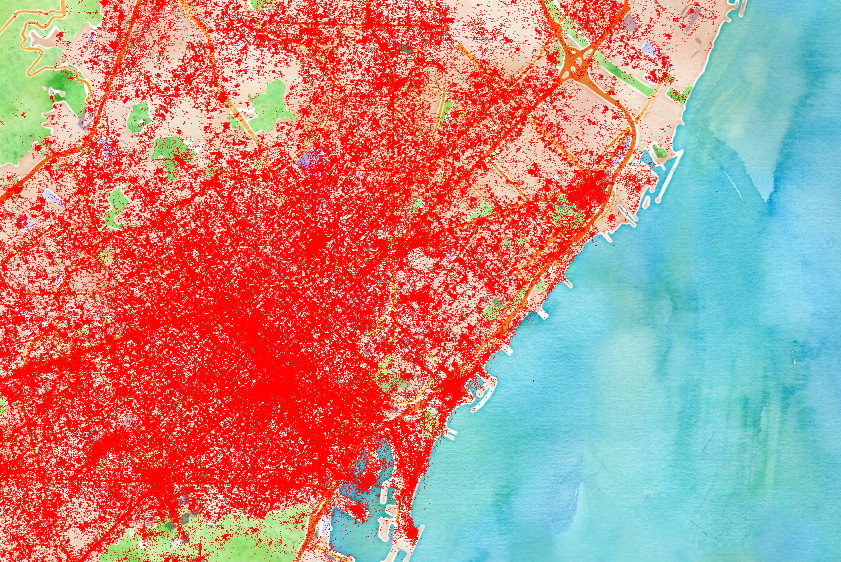
\includegraphics[scale=0.2]{bigdata1.png}  
%}
%\end{titlepage}

\end{frame} 
 
\begin{frame}
\begin{figure}
  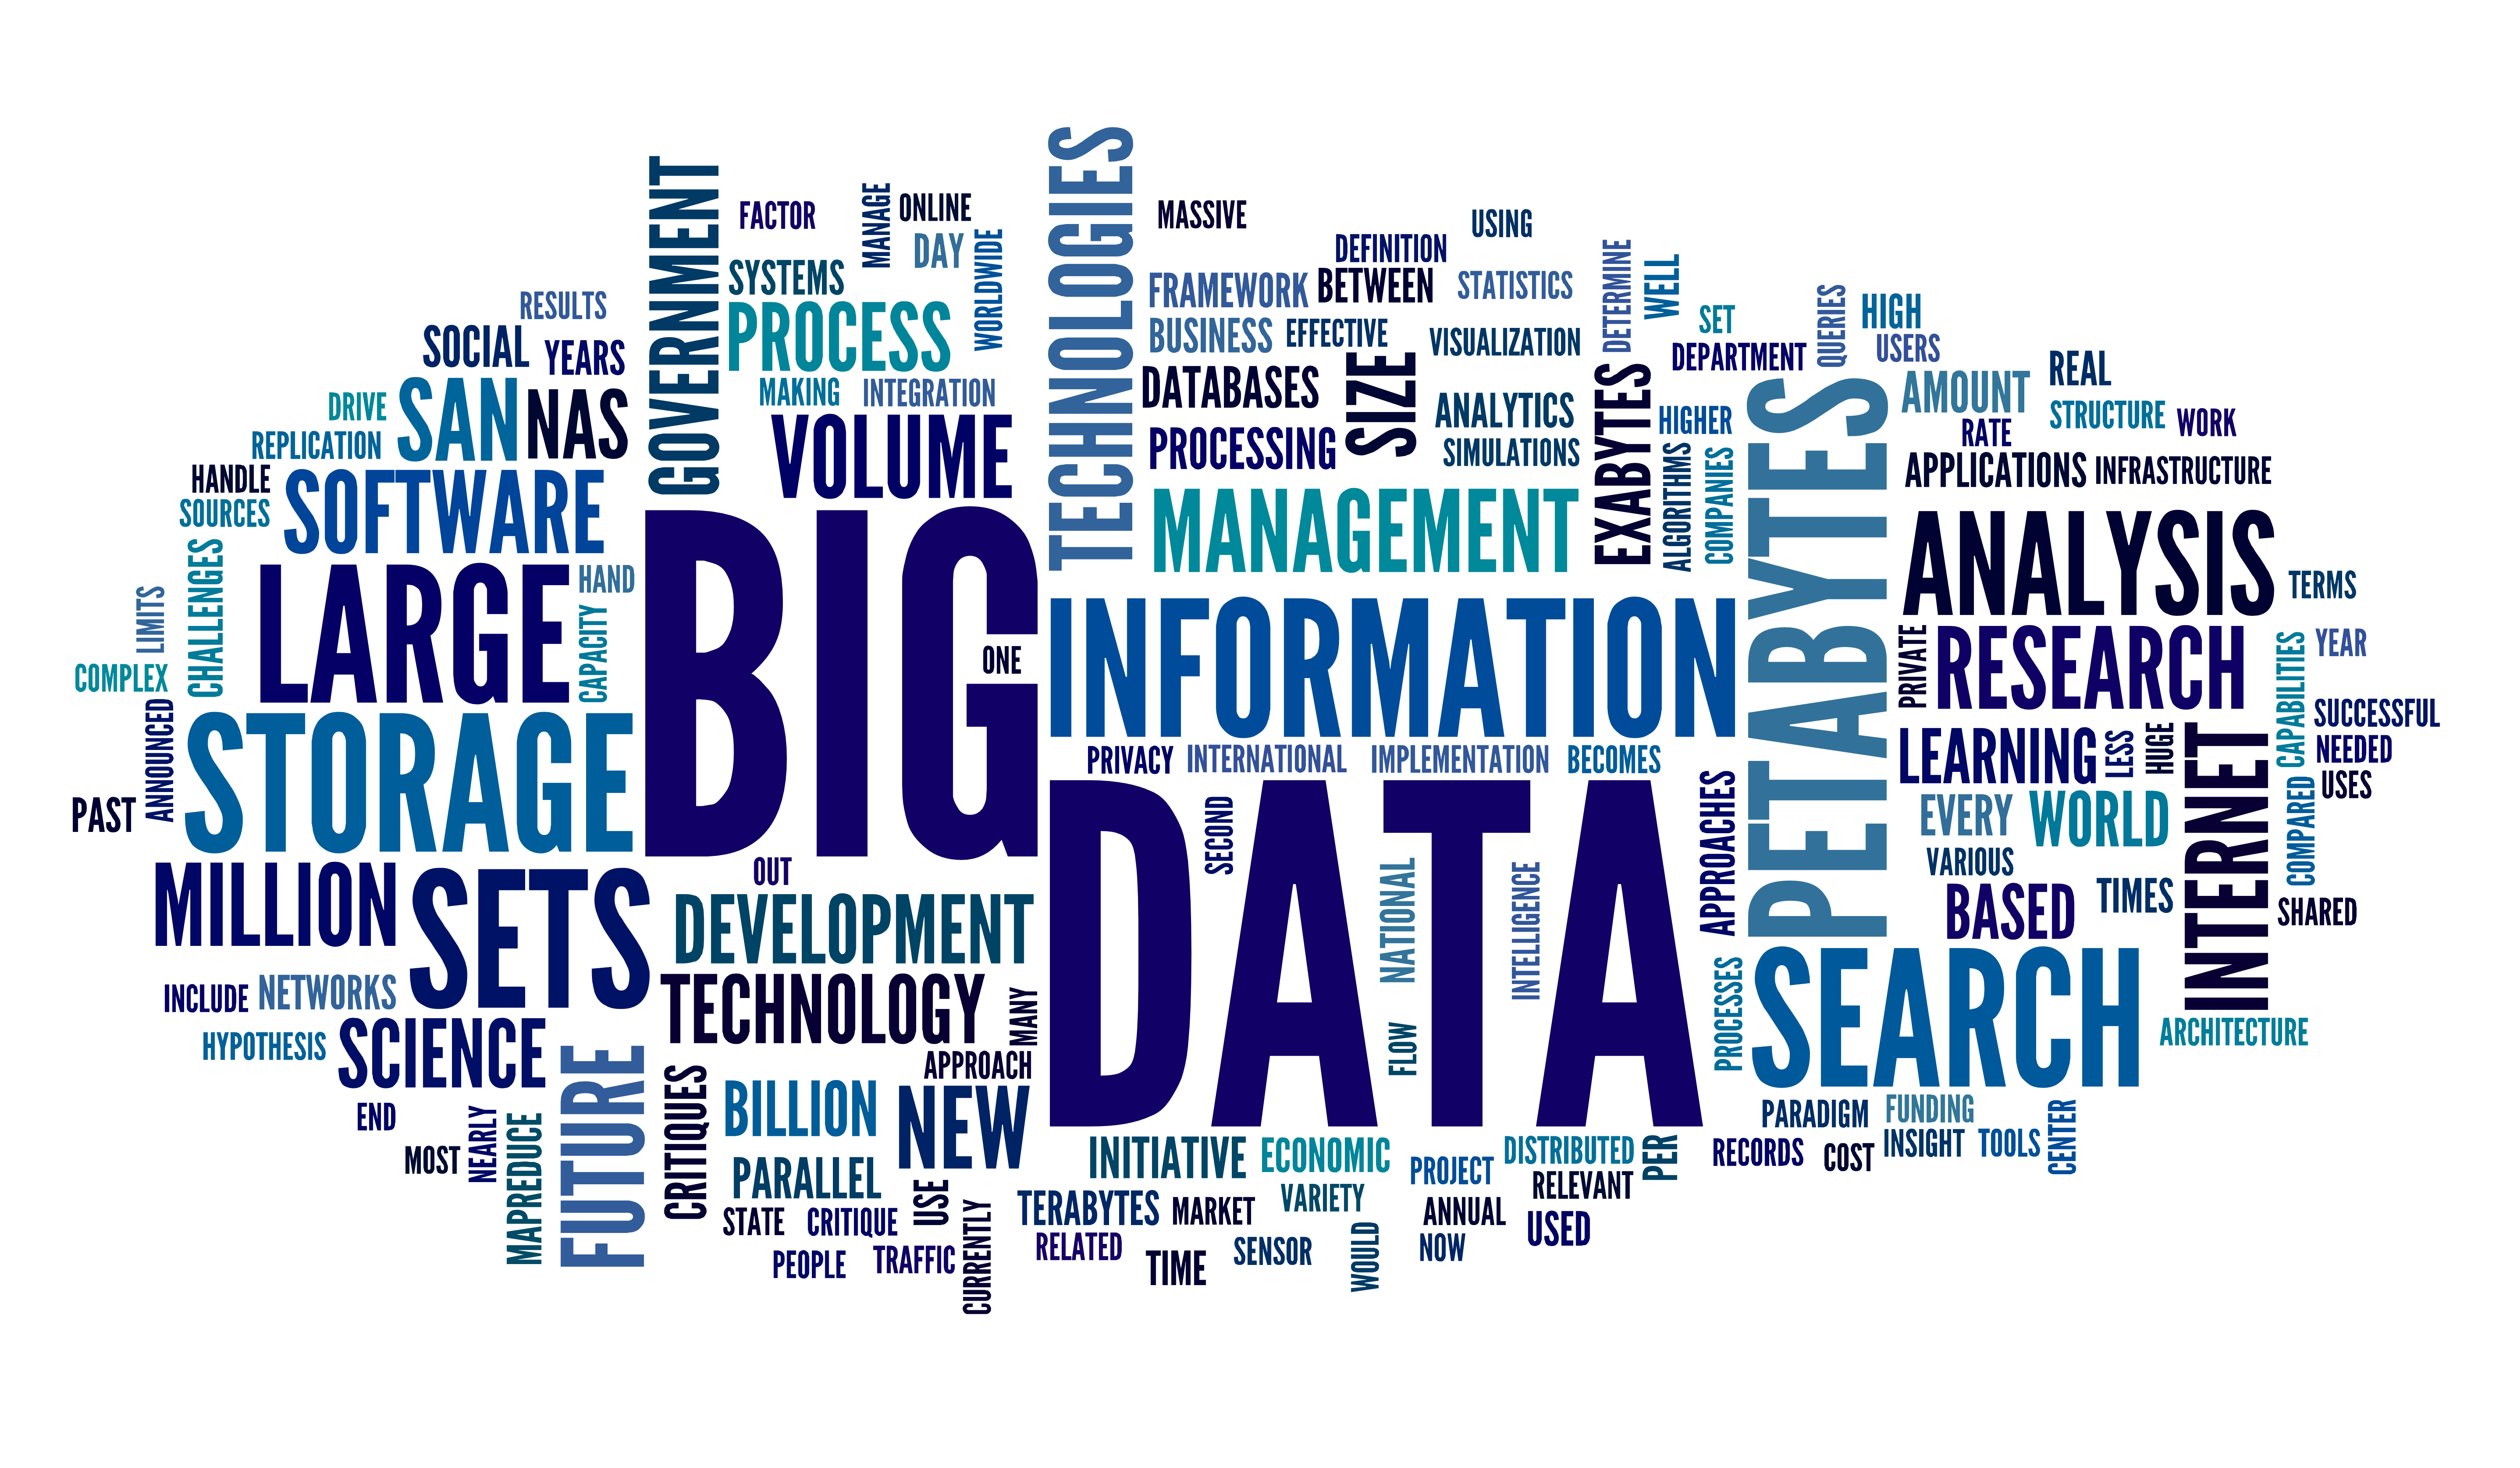
\includegraphics[width=\textwidth]{wordcloud.jpg}
\end{figure}
\tiny{Big Data Word Cloud; source:\url{http://olap.com/big-data/}}
\end{frame} 
 
 
\begin{frame}
\frametitle{Table of Contents}
%\tiny{
\tableofcontents%}
\end{frame}

\begin{frame}
\frametitle{Warning}
\begin{figure}
  
\includegraphics[scale=0.40]{warning.jpeg}
\end{figure}
\textbackslash *
This presentation may contain tech talk, such as: databases, clusters, NoSQL.\\
If you are susceptible to these concepts, you may want to leave the room \textbf{now}.\\
From this point beyond, you are at your own risk!
\textbackslash *
\end{frame}

\section{The Value of Data} 
\begin{frame}
\frametitle{The Value of Data}
%Not a new idea
\textbf{Not a New Idea!}
\begin{columns}
  \begin{column}{0.5\textwidth}  
    \begin{itemize}
      \item<1->Matthew Fontaine Maury (1806-1873).
      \item<2->Foresaw the hidden value on captain's ships logs, when analysed collectively.
      \item<2->Used time series data to carry out analysis that would enable him to recomend optimal shipping routes.%based on winds and currents      
      \end{itemize}
  \end{column}
  \begin{column}{0.5\textwidth}    
    \begin{figure}
    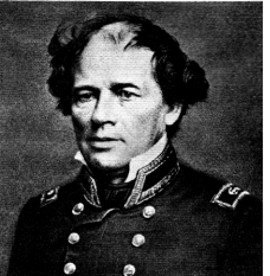
\includegraphics[scale=0.40]{maury.jpg}
    \end{figure}    
  \end{column}  
\end{columns}
%American sailor,
%A leg injury turned him to study meteorology, astrology, oceanography, cartography
\end{frame}

%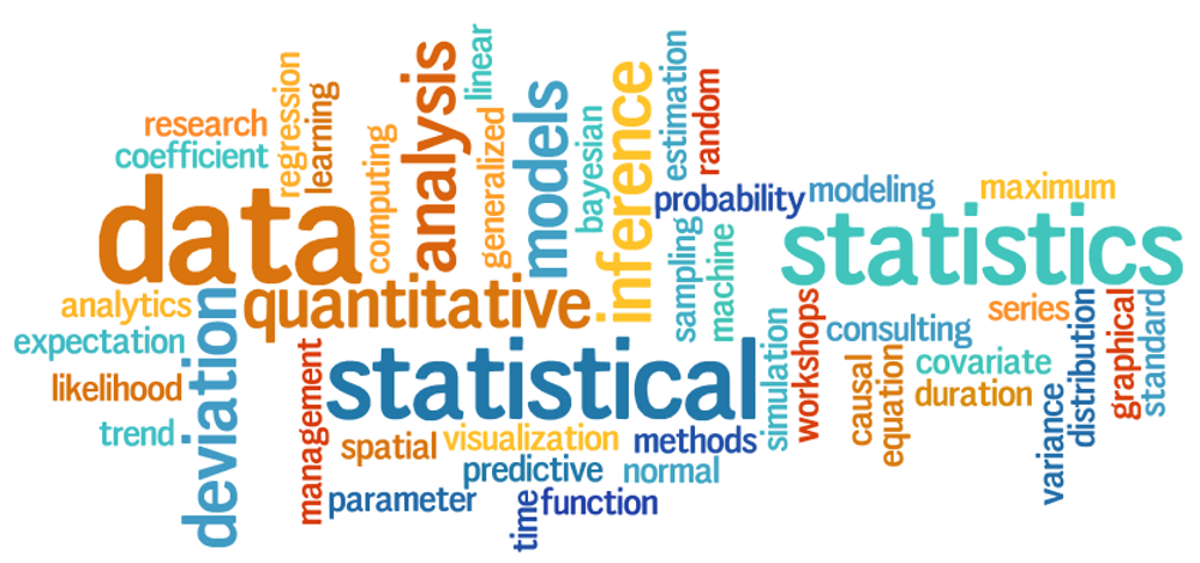
\includegraphics[scale=0.2]{wordcloud_ds.png}\\
%sexiest job of the 21st Century’ 
%\tiny{Data Science Word Cloud; source:\url{http://data.library.virginia.edu/statlab/}}

\begin{frame}
\frametitle{The Value of Data}
\textbf{Data Mining, Open-source and Crowd-sourcing}
\small{
    \begin{itemize}
      \item<2->In 1848, Captain Jackson was the the first person to try the route recommended by Maury, and as a result he was able to save 17 days on his outbond trip.
      \item<3->Apart from collecting existing logs, Maury encouraged the collection of more regular and systematic time series, by creating a template.
      \item<4->Collected Data: longitude, latitude, currents, magnetic variation, air and water temperature, general wind direction, etc.      
      \end{itemize}
}
    \begin{figure}
      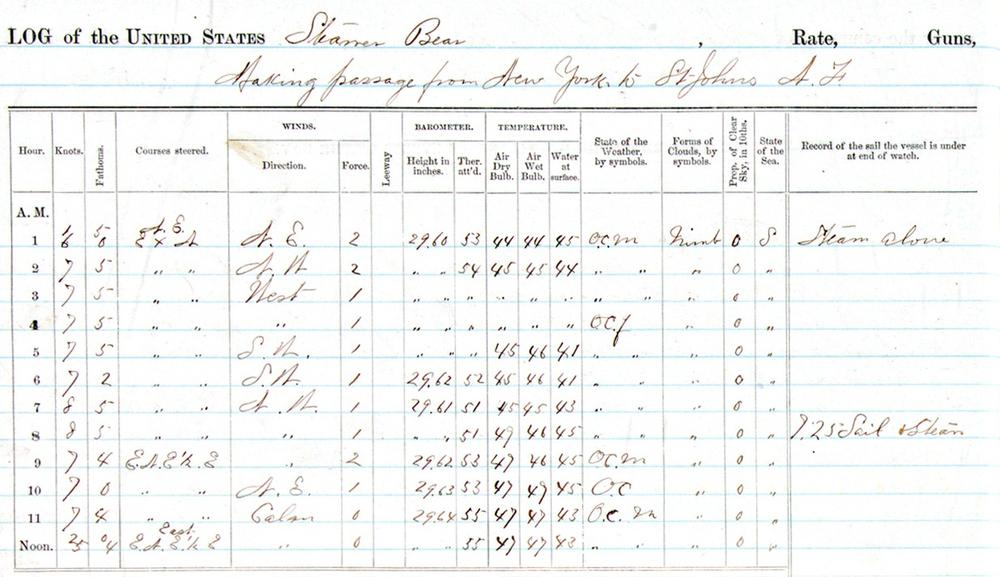
\includegraphics[scale=0.15]{log.jpg}
     \end{figure}
\end{frame}

\begin{frame}
\frametitle{Data Analysis}
\textbf{A multidisciplinary field}
    \begin{figure}
      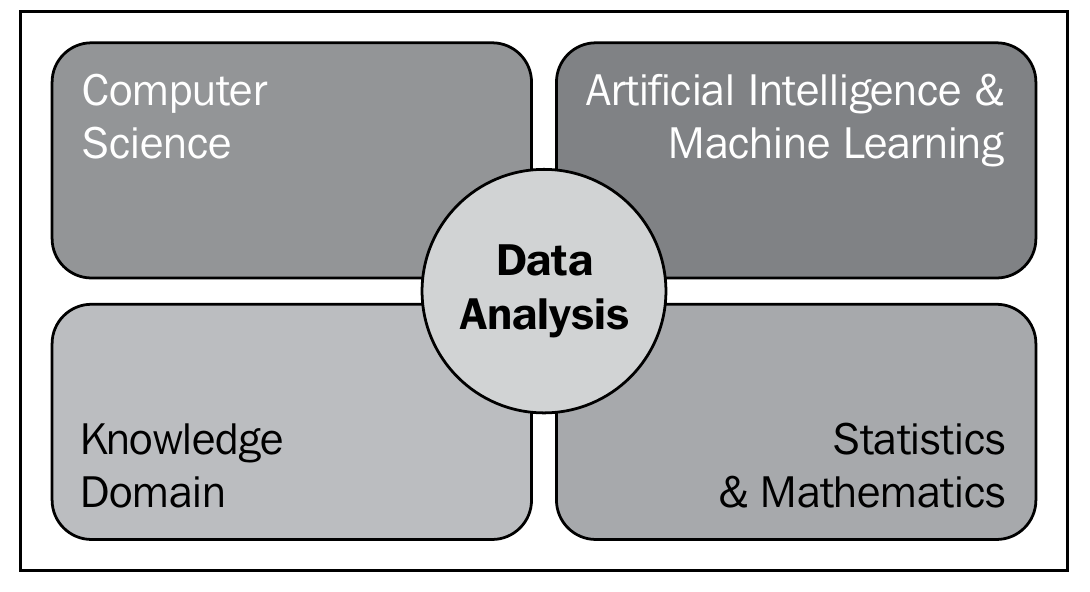
\includegraphics[width=0.8\textwidth]{data_analysis.png}
     \end{figure}
\end{frame}

\begin{frame}
\frametitle{Data Analysis}
%In the past few years, this is what people were using
\textbf{Traditional Stack}
    \begin{itemize}
      \item Spreadsheets (e.g.: Excel, OpenOffice)
      \item RDBMS (e.g.: Oracle, PostgreSQL, MySQL)
      \item Statistical Packages (e.g.: R, Matlab)
      \item GIS Packages (e.g.: QGIS)      
      \item Scripting and programming languages (e.g.: Python, Java)
      \item Libraries      
      \end{itemize}  
\end{frame}

\section{The Big Data Revolution}
\begin{frame}
\frametitle{Big Data}
\textbf{What changed in recent years?}
   \begin{itemize}
      \item Differences in the way global business and transportation are done have exploded the volume of traditional data sources.%a much larger scale for traditional types of data
      \item Widespread increase in data from sensors. %Internet of things: wide arrays of machines that report back to servers or communicate directly with each other
      \end{itemize}
      \vspace{5mm}
    \begin{figure}       
	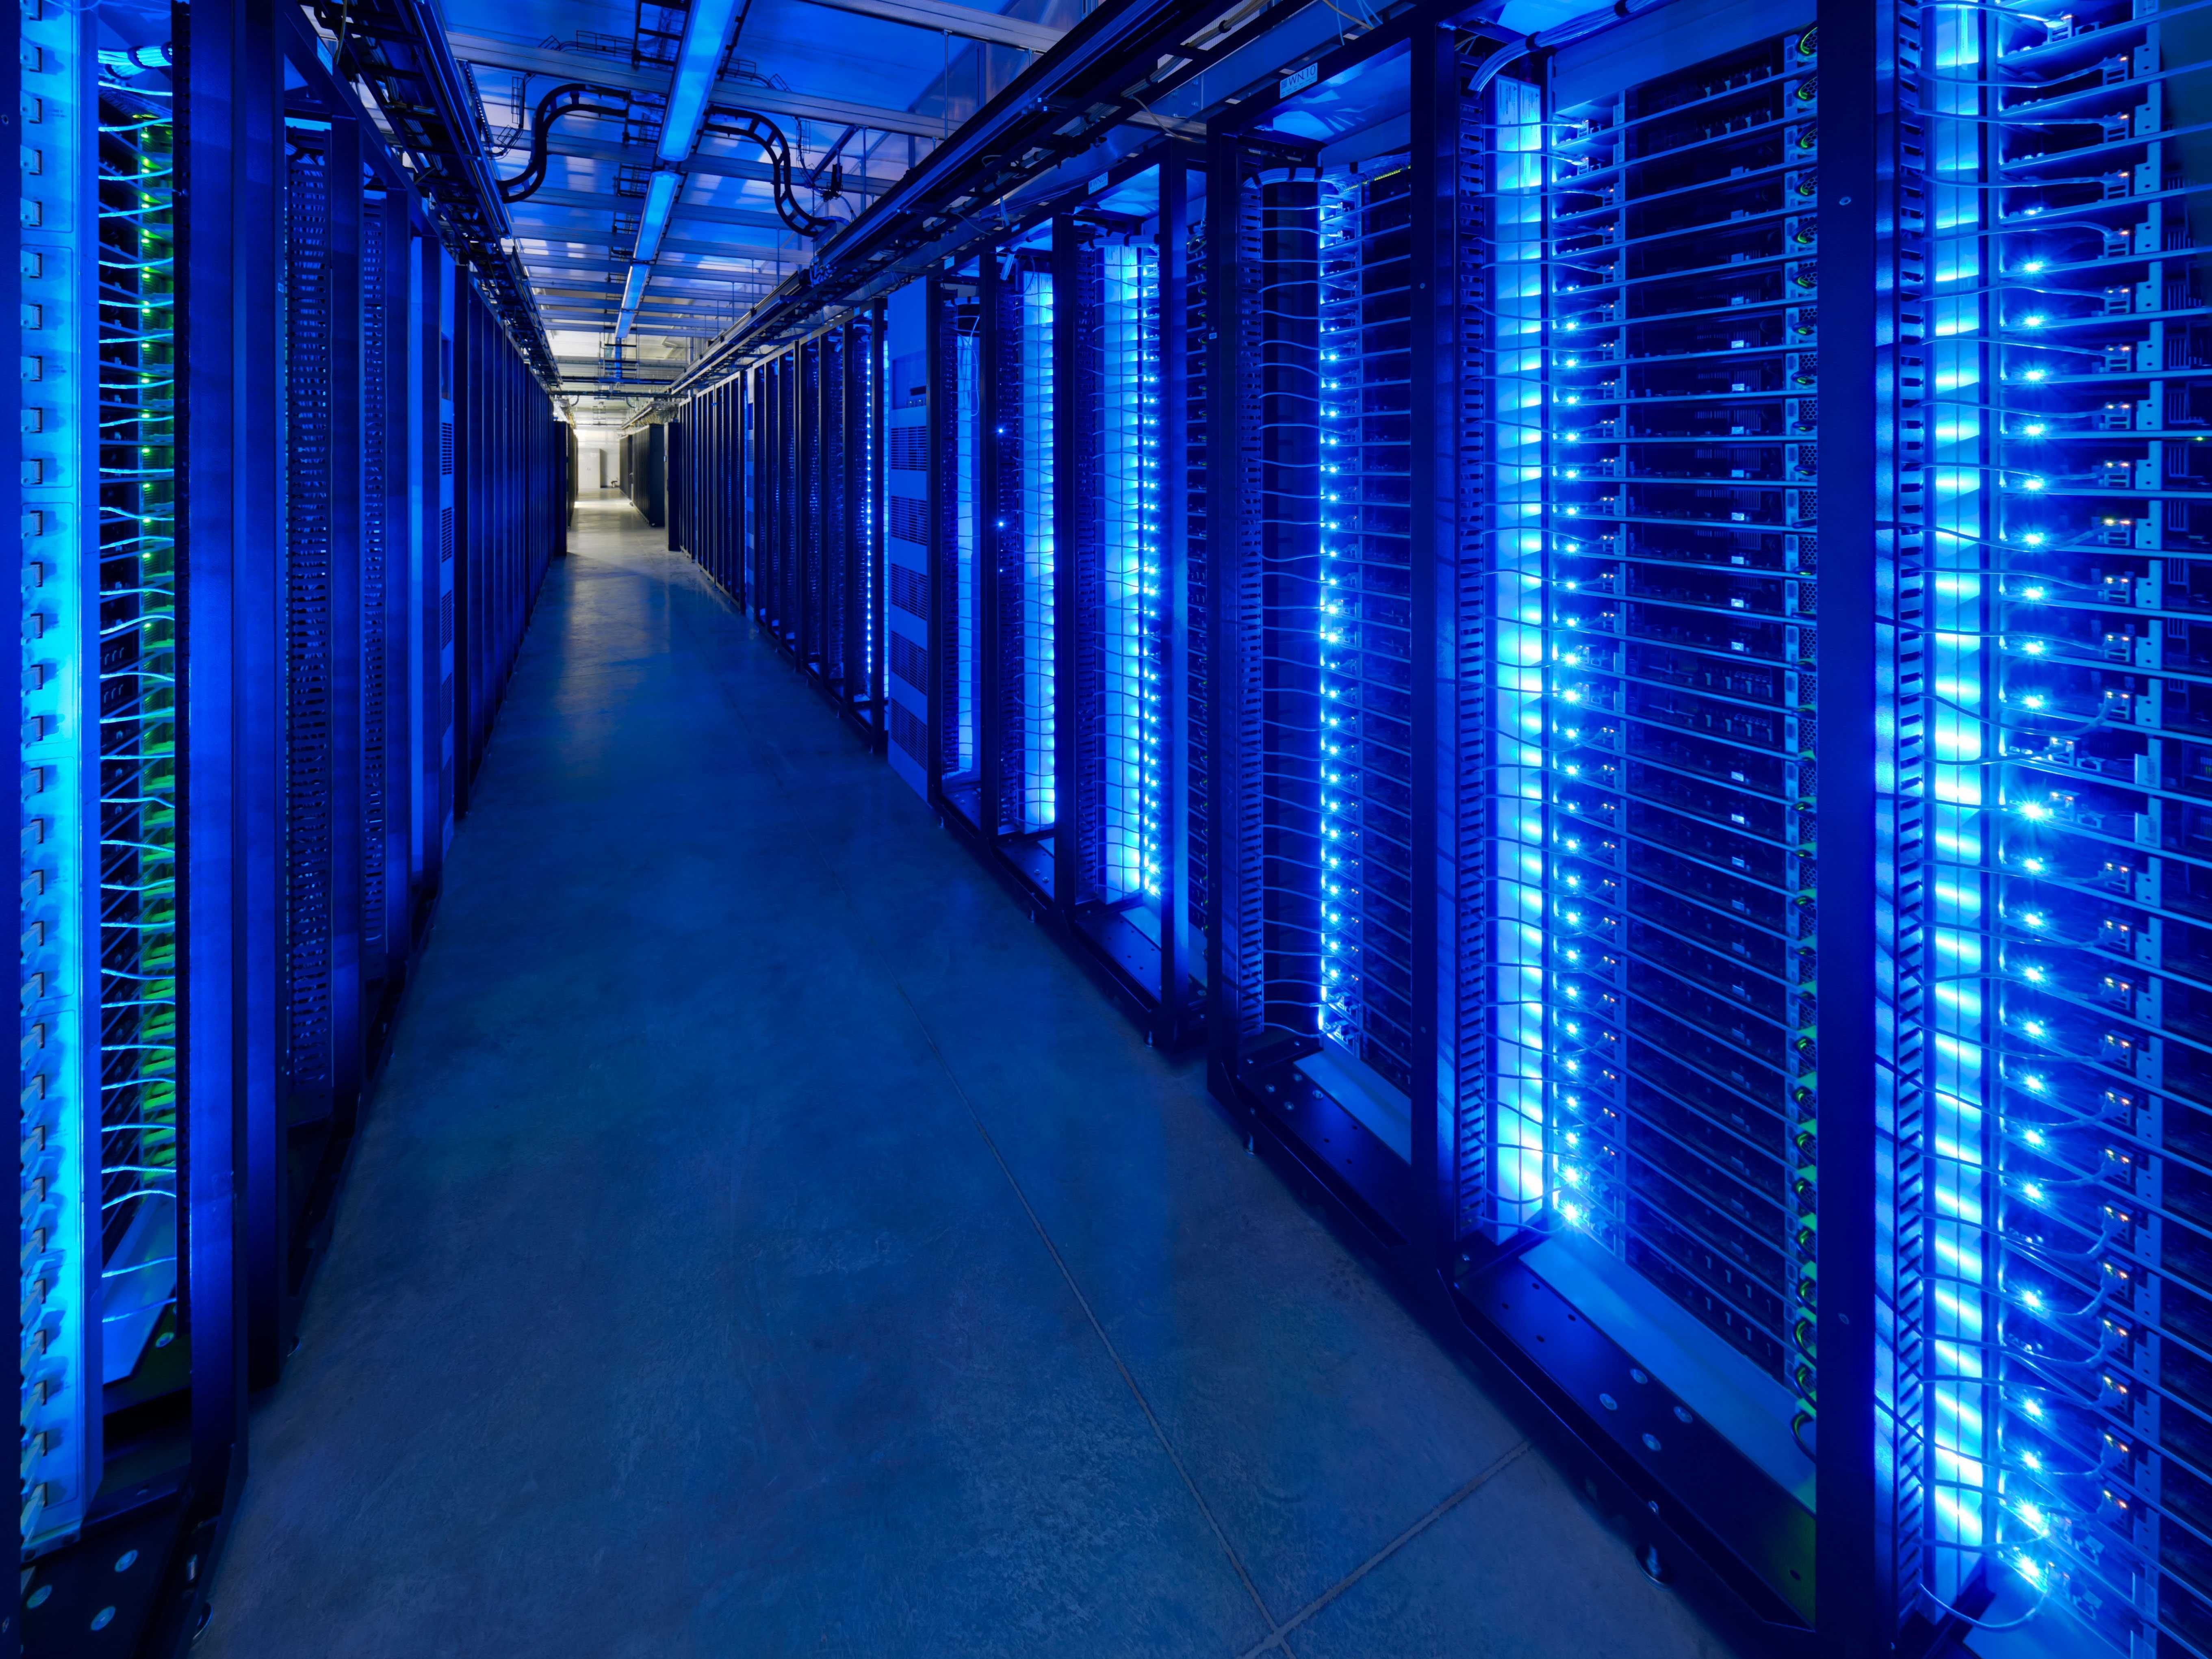
\includegraphics[width=0.4\textwidth]{cluster.jpg}      
     \end{figure}
\end{frame}


\begin{frame}
\frametitle{Big Data}
\textbf{Smart Citizen Project}
\begin{columns}
  \begin{column}{0.5\textwidth}\small{ 
    \begin{itemize}
      \item<2->Platform to generate participatory processes of people in the cities, by connecting data, people and knowledge.
      \item<3->Based on geolocation, Internet and free hardware and software for data collection and sharing.
      \item<4->Relies on the production of objects to connect people with their environment and their city.     
      \end{itemize}  }
  \end{column}
  \begin{column}{0.5\textwidth}
    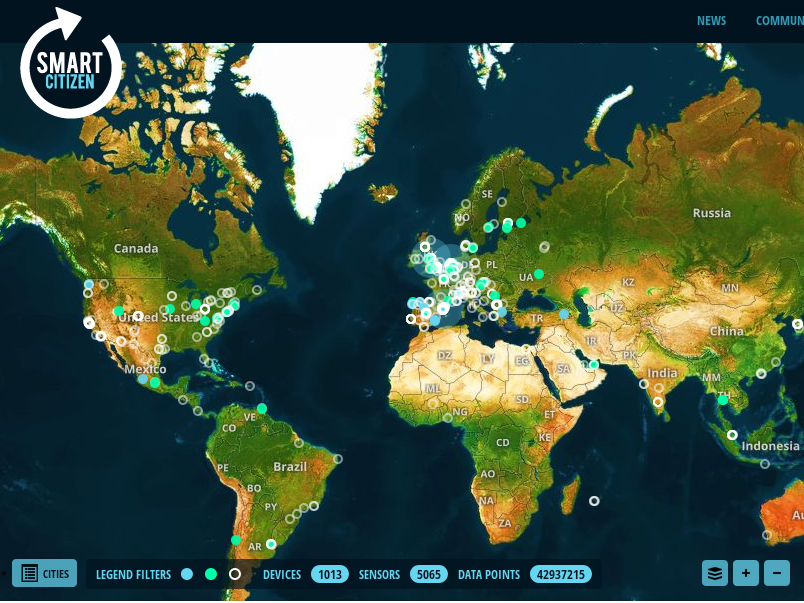
\includegraphics[width=\textwidth]{smart_city.png}\\
    %Although it initally started in BCN (FabLab), these crowd sourcing data collection structures have the potential to increase exponentially.
    \tiny{\url{https://smartcitizen.me/}}  
  \end{column}  
\end{columns}
\end{frame}

\begin{frame}
\frametitle{Big Data}
\small{
    \begin{itemize}
      \item<2->A great deal of this data is actually geo-located (e.g.: satellite navigate coordinates, ip addresses). % satellite navigation
      %Unlike other sciences (e.g.: astronomy,medicine) till recently geography suffered from the lack of available spatial data.
      \item<3->Geography has finally the opportunity to switch from being based on guesses and samples, to become a truly data-driven science.
      \end{itemize}
}

\begin{columns}
  \begin{column}{0.5\textwidth}
      \begin{figure}       
	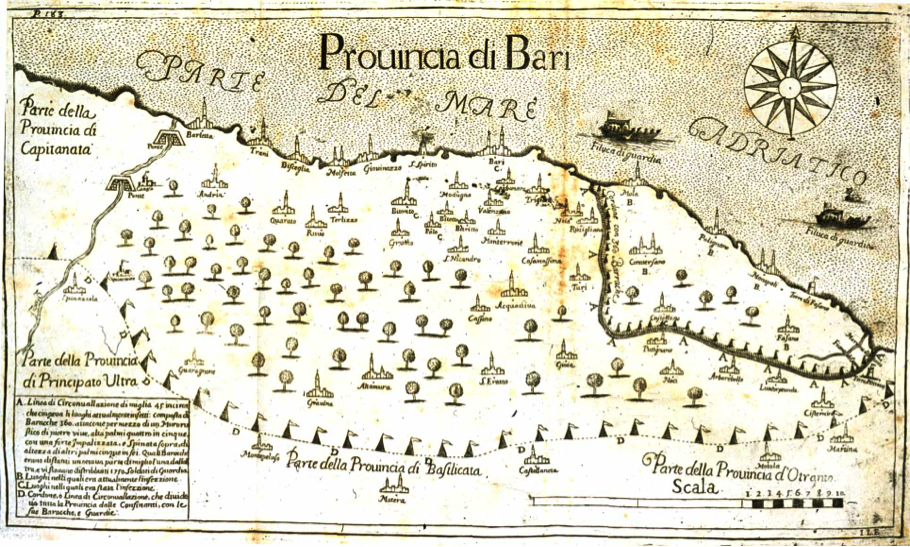
\includegraphics[width=\textwidth]{old_map.png}      
     \end{figure}
    \tiny{Based on reports, Fillipo Arrieta published maps describing a multi-stage containment plan designed to limit the plague in Bari (1864).}
  \end{column}
  \begin{column}{0.5\textwidth}
    \begin{figure}       
	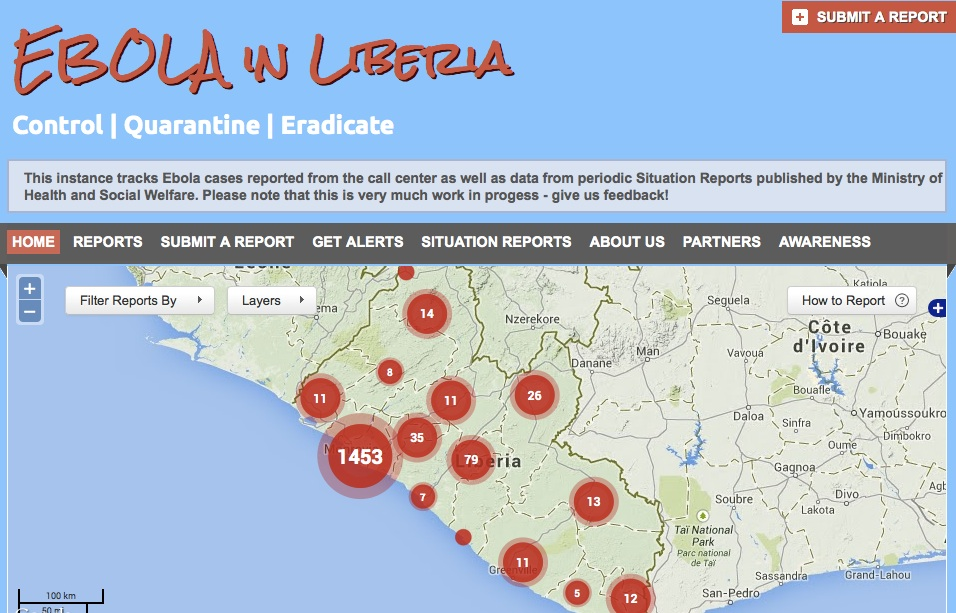
\includegraphics[width=\textwidth]{ebola_ushahidi.jpg}      
     \end{figure}
    \tiny{The iLab used the ushahidi platform to collect and display crowd-sorcing information about Ebola in Liberia (2014).}  
  \end{column}  
\end{columns}

%In 1694 Bari, Italy administrator Fillipo Arrieta published two maps that carefully detailed a multi-stage containment plan designed to limit plague incursions in Bari, Italy.
\end{frame}

\begin{frame}
\frametitle{Big Data}
\textbf{What characterizes Big Data?}%3vs
    \begin{itemize}
      \item<2->\textbf{Volume}: Large amounts of data.
      \item<3->\textbf{Variety}: Different types of structured, unstructured, and multi-structured data.
      \item<4->\textbf{Velocity}: Needs to be analyzed quickly.
      \end{itemize}
    \begin{figure}       
	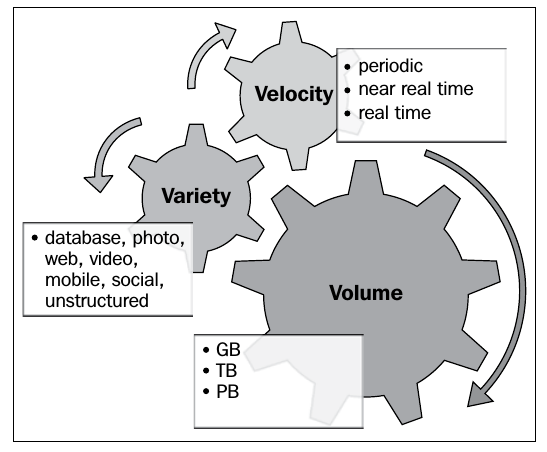
\includegraphics[width=0.4\textwidth]{3vs.png}      
     \end{figure}      
\end{frame}

\begin{frame}
\frametitle{Technological Challenges}
These characteristics map into challenges:
    \begin{itemize}
      \item Scalability %horizontal scalability vs vertical scalability
      \item Heterogeneity % different data sources, with completely different structure
      \item Low latency % real time
      \end{itemize}
\vspace{5mm}      
When the traditional stack is no longer enough, a paradigm shift is required.
\begin{figure}   
  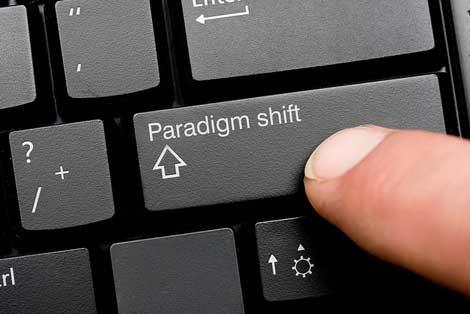
\includegraphics[width=0.3\textwidth]{paradigm_shift.jpg}   
\end{figure}   
%spatial working on the edge
\end{frame}

\begin{frame}
\frametitle{RDBMS vs NoSQL}
%Relational Model formulated by Codd in 1970, represents reality through: tables, rows and columns.

    \begin{figure}   
      
\includegraphics[width=0.2\textwidth]{nosql.jpg}   
    \end{figure}    
    
    \begin{itemize}    
      \item<2->NoSQL databases trade away some capabilities of relational databases (SQL), in order to improve scalability.%SQL language and optimizer
      \item<3->Advantages: NoSQL databases are simpler, can handle semi-structured and denormalized data and have an higher scalability.
      \item<4->Disadvantages: loss of abstraction provided by the query optimizer, that increases the complexity of the applications.% the logic is implemented and optimized in the application, an extra burden for the developer
      \item<5->Recently, tools were developed that bring back the full power of SQL language to the NoSQL ecosystem (e.g.: Apache Drill, Hive).      
      \end{itemize}
\end{frame}


\begin{frame}
\frametitle{RDBMS vs NoSQL}
    \begin{figure}   
      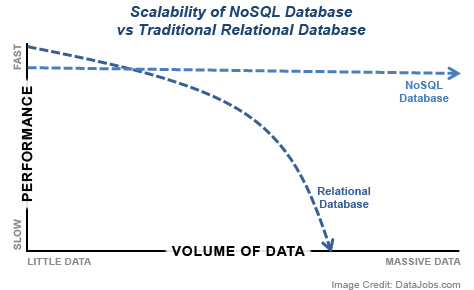
\includegraphics[width=0.8\textwidth]{sql_vs_nosql.jpg}   
    \end{figure}         
\end{frame}

\begin{frame}
\frametitle{Examples}
    \begin{figure}   
      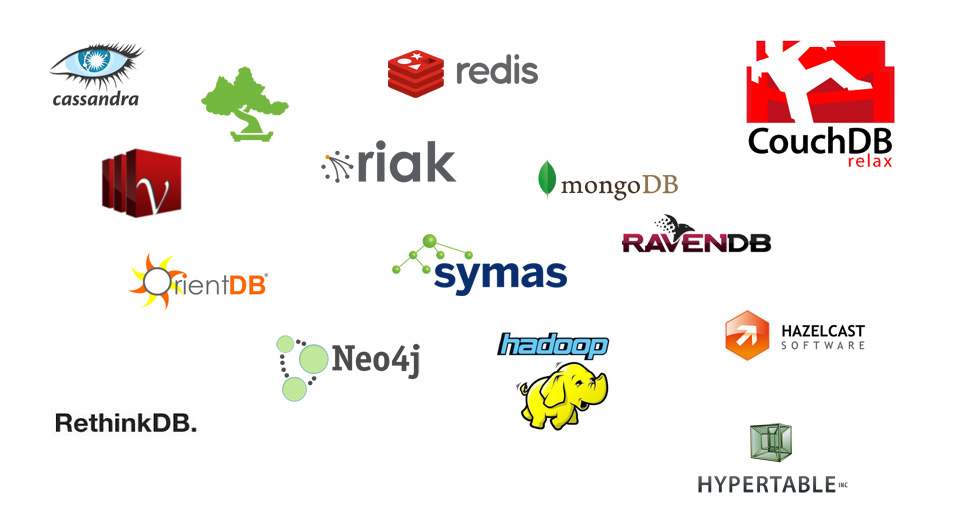
\includegraphics[width=\textwidth]{examples.jpg}%key value,columnar, big table, document, graph   
    \end{figure}    
\end{frame}

\begin{frame}
\frametitle{MapReduce}
Programming model for processing and generating large data sets with a parallel, distributed algorithm on a cluster.
%It is basically composed by two operations, inspired by functional programming
    \begin{itemize}    
      \item<1->Map(): performs filtering and sorting.%such as sorting students by first name into queues, one queue for each name
      \item<1->Reduce(): performs a summary operation. % such as counting the number of students in each queue, yielding name frequencies
      \item<2->The framework coordinates the processing, by marshalling the distributed servers, running the tasks and parallel and managing all communications and data between the various parts of the system.% true parallel system, that can be deployed on the cloud
      \item<3->There are many libraries that implement MapReduce.%Apache Hadoop is a popular Free and Open-Source implementation.
      \end{itemize}
\end{frame}

\begin{frame}
\frametitle{A Big Data Approach}

\textbf{Does this mean we have to throw away our traditional tools and methods?}

%not really. mix and match
    \begin{itemize}    
      \item<2->First ensure that you \textbf{really} have, or will have Big Data at some point in the future.%scalability requirement. Don't go for this approach, for instance if you are working with a small static data sample, that you can approach with a traditional stack (example: number of voters in a local election 2014)
      \item<3->Then identify the stages of the workflow that are bottlenecks, in terms of the current technologies.%Most often you will not have Big Data all along the workflow, and nearly always the results of a Big Data workflow are not Big Data (we want to achieve dimensionality reduction).
      \item<4->It is possible to mix \& and match.%To have a mixed stack combining SQL and noSQL technologies
      \end{itemize}
\end{frame}


\section{An Use Case}
\begin{frame}
\textbf{Analysing geo-located Tweets}
    \begin{itemize}    
      \item<2->The purpose of this use case was to analyse the stream of geo-located Tweets, as a sensor for citizen presence.
      \item<3->Number of tweets in Catalunya in around 3 months: +- 6 million.
      \item<4->Continuous stream of data.%This value is increasing everyday.
      \item<5->This amount of data is not easily assimilated by the "human-eye", so we decided to create clusters of Tweets.
     \end{itemize}
      \begin{figure}   
      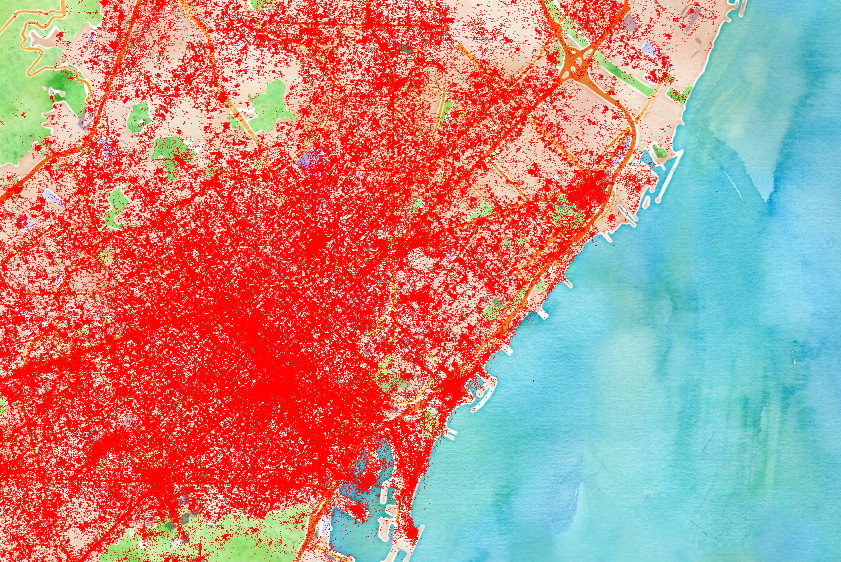
\includegraphics[width=0.4\textwidth]{bigdata1.png}   
     \end{figure}       
\end{frame}

\begin{frame}
\frametitle{An Use Case}
\textbf{Clustering}
    \begin{itemize}    
      \item<2->It is a descriptive data mining technique, often used for dimensionality reduction.
      \item<3->It groups a set of objects in such a way that objects in the same group are more similar to each other, than to object in other groups.
      \item<4->Strictly, it corresponds to a family of unsupervised machine learning algorithms.
      \item<5->We wanted to implement this concept using only Hadoop, and apply it to spatial attributes.%No ML libraries (Mahout)
     \end{itemize}
\end{frame}

\begin{frame}
\frametitle{Technological Stack}
      \begin{figure}   
      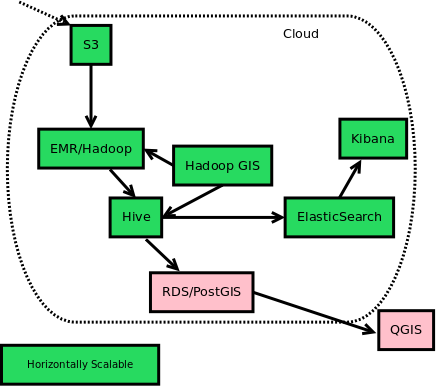
\includegraphics[width=0.7\textwidth]{stack.png}   
     \end{figure}       
\end{frame}

\begin{frame}
\frametitle{Workflow}
      \begin{figure}   
      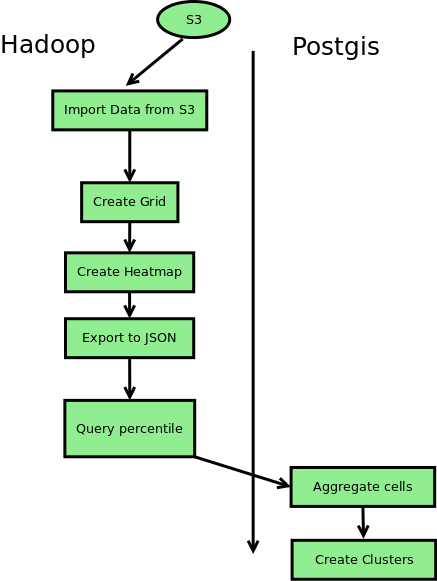
\includegraphics[width=0.5\textwidth]{geo3.png}   
     \end{figure}       
\end{frame}

\begin{frame}
\frametitle{Results}
Using this workflow we were able to turn the original point cloud, into a density grid, and then into clusters.
\begin{columns}
  \begin{column}{0.5\textwidth}
      \begin{figure}       
	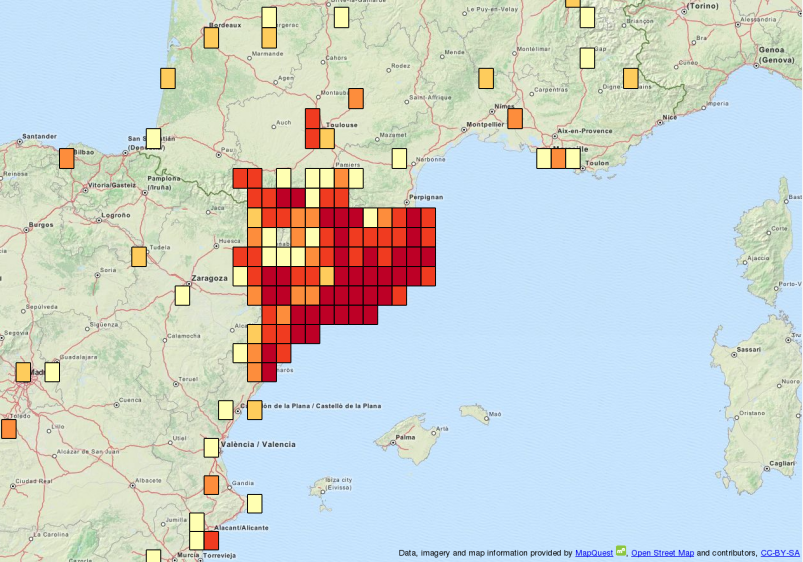
\includegraphics[width=\textwidth]{heatmap_hive.png}      
     \end{figure}
  \end{column}
  \begin{column}{0.5\textwidth}
    \begin{figure}       
	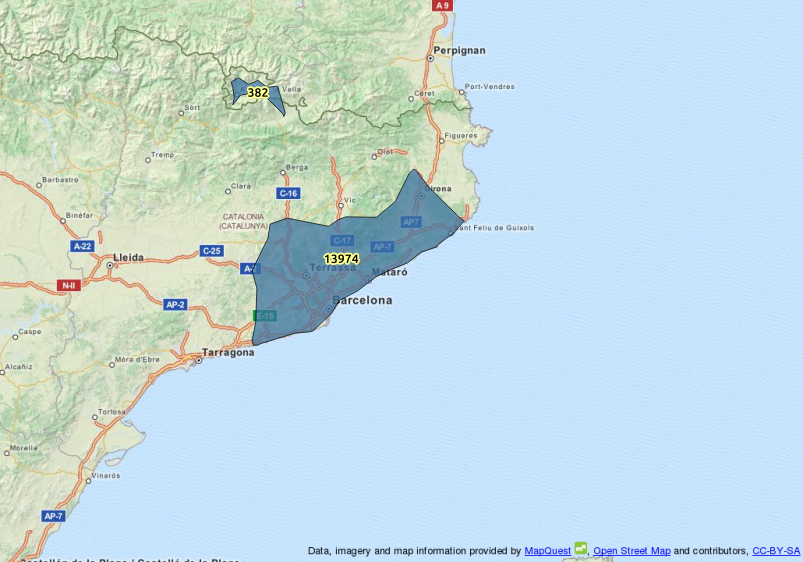
\includegraphics[width=\textwidth]{clusters_hive.png}      
     \end{figure}
  \end{column}  
\end{columns}
      \vspace{5mm}  
Clusters expose patterns of presence over time, and can help us to re-define boundaries for the city that are data-driven, rather than administrative.%bottom up vs top-down
%As we identified and solved the bottlenecks with the relevant tools, in theory this algorithm is scalable to any Petabytes of data.%quadrillions of bytes
\end{frame}

\section{Final Remarks}
\begin{frame}
\frametitle{Final Remarks}
    \begin{itemize}    
      \item<2->It is ok to use non scalable tools, at certain points of the workflow.
      \item<3->We are working on the edge of existing technologies; some functions were not implemented yet, and bugs are common.
      \item<4->Since it is a niche, this is even more true for spatial technologies.
      \item<5->There are not ready-made solutions: the particular stack and workflow should be compiled for the specific case study.
      \item<6->this is one stack to solve this problem; it is not the only one, and it may not even be the "best" one;% if such a things exists
     \end{itemize}
\end{frame}


\begin{frame}
\frametitle{Acknowledgements}
I would like to thank Ellen Friedman (MapR, Apache Mahout, Apache Drill), for her inspiring work on Big Data and Machine Learning.
    \begin{figure}   
      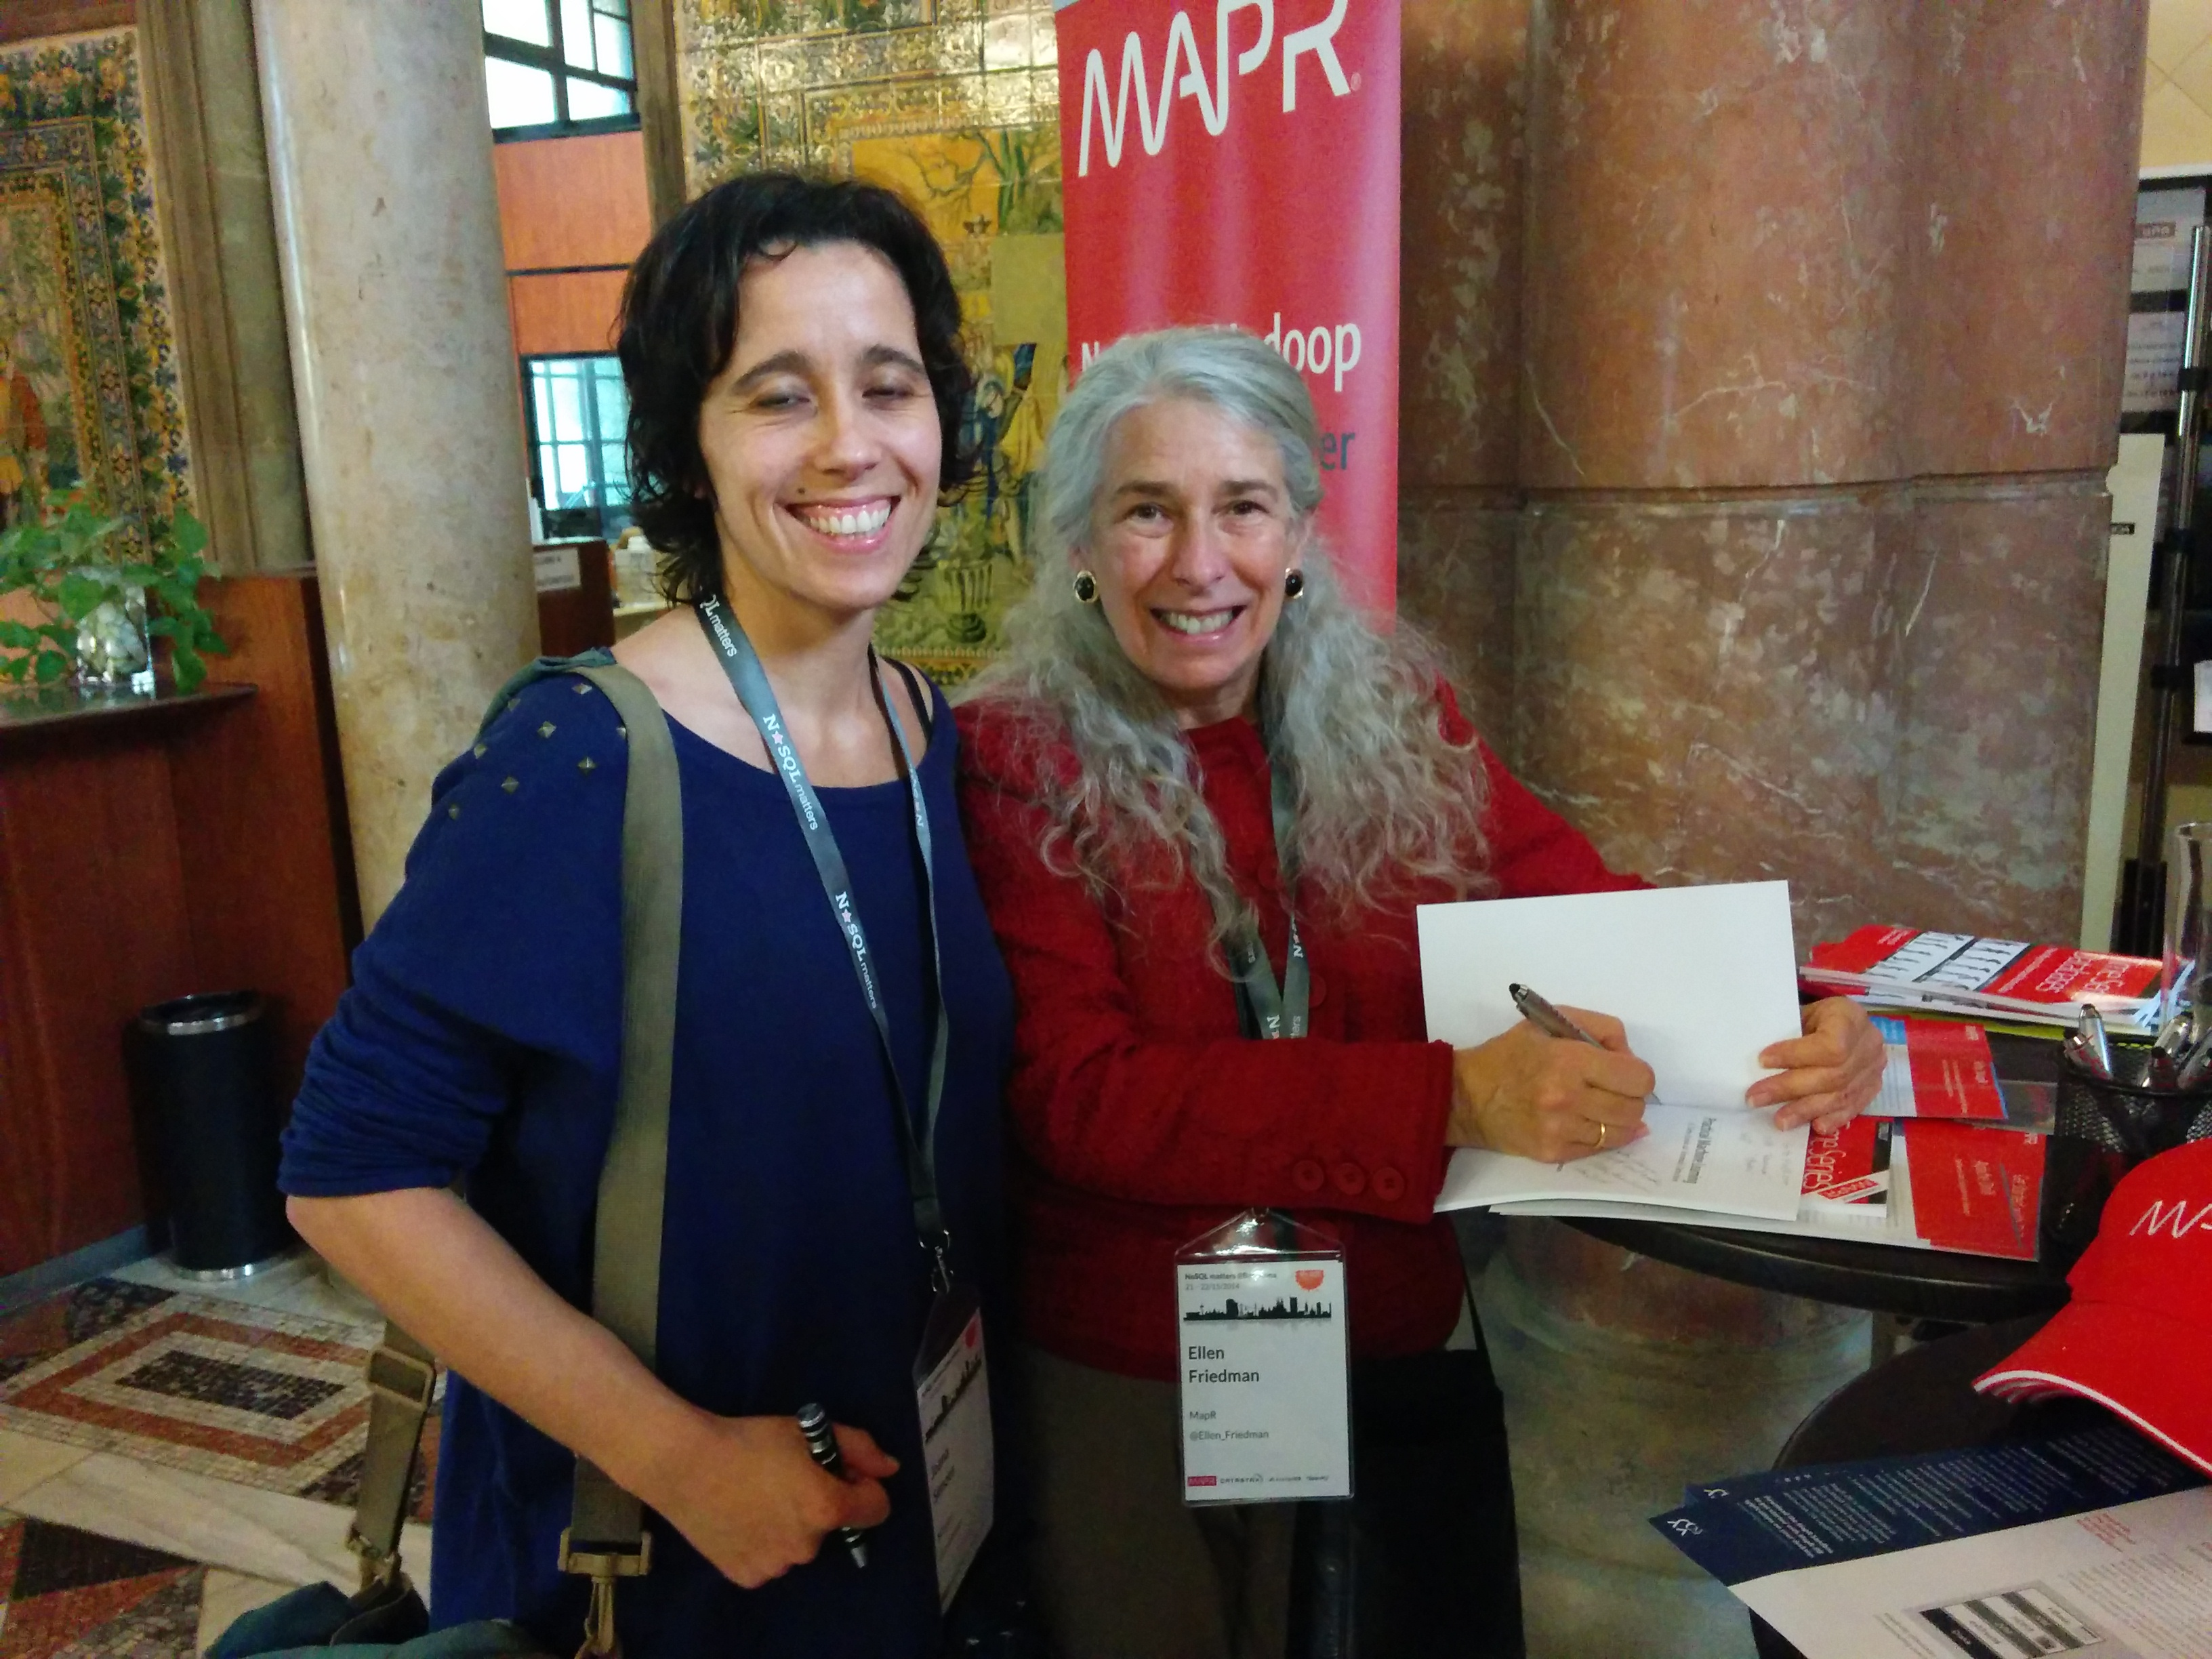
\includegraphics[width=0.7\textwidth]{nosql_matters.jpg}      
    \end{figure}   
\end{frame}

\begin{frame}
\frametitle{References}
\begin{itemize}
\item Aji, A., Wang, F., Vo, H., Lee, R., Liu, Q., Zhang, X. and Saltz, J." Hadoop-GIS: A High Performance Spatial Data Warehousing System over MapReduce". Proceedings of the VLDB Endowment International Conference on Very Large Data Bases, 6(11), p1009. (2013)
\item Cuesta, H. "Practical Data Analysis". Packt Publishing (2013)
\item Dunning, T. and Friedman, E. "Time Series Databases: New Ways to Store and Access Data". O'Reilly Media; 1 edition (October, 2014)
\item Myatt, G and Johnson, W. "Making Sense Of Data I: A Practical Guide to Exploratory Data Analysis and Data Mining". O'Reilly : 2 edition (2014).
\end{itemize}
\end{frame}

\begin{frame}
\frametitle{Thank You!}
    \begin{figure}   
      
\includegraphics[width=0.2\textwidth]{thanks.jpg}      
    \end{figure}   
    This presentation is available at: \centering{\\ \url{http://tinyurl.com/pcmgzxp}\\}
      \vspace{5mm}    
    Next:
    \begin{itemize}    
      \item<2-> 9as Jornadas de SIG Libre -  26th-27th March 2015, Girona.
     \end{itemize}
\end{frame}

\end{document}